% This is samplepaper.tex, a sample chapter demonstrating the
% LLNCS macro package for Springer Computer Science proceedings;
% Version 2.20 of 2017/10/04
%
\documentclass[runningheads]{llncs}
%
\usepackage{float}
\usepackage{graphicx}
\usepackage{balance}
\usepackage{color}
\usepackage{amsmath}
\newcommand{\trishita}[1]{{\color{magenta}\bfseries[Trishita: #1]}}
% Used for displaying a sample figure. If possible, figure files should
% be included in EPS format.
%
% If you use the hyperref package, please uncomment the following line
% to display URLs in blue roman font according to Springer's eBook style:
% \renewcommand\UrlFont{\color{blue}\rmfamily}
\begin{document}
%
\title{Distributed Ethereum Web Browser Mining\thanks{Supported by organization x.}}
%
%\titlerunning{Abbreviated paper title}
% If the paper title is too long for the running head, you can set
% an abbreviated paper title here
%
\author{Trishita Tiwari\orcidID{0000-1111-2222-3333} \and
David Starobinski\orcidID{1111-2222-3333-4444} \and
Ari Trachtenberg\orcidID{2222--3333-4444-5555}}
%
\authorrunning{T. Tiwari et al.}
% First names are abbreviated in the running head.
% If there are more than two authors, 'et al.' is used.
%
\institute{Boston University, Department of Electrical and Computer Engineering, Boston, MA 02215, USA \\
\email{\{trtiwari,staro,trachten\}@bu.edu}}
%
\maketitle             
%
\begin{abstract}
Given the seemingly endless growing popularity of crypto-currencies, there is an increasing interest in different mining possibilities. This paper proposes a web browser based mining implementation for Ethereum implemented both in JavaScript and WebAssembly to perform the necessary Proof-of-Work (PoW) computations to mine the Ethereum blockchain. We explore a variety of techniques to distribute the inherently memory and memory intensive PoW of Ethereum over multiple browser-based clients that have limited resources. We obtain the best results with the WebAssembly implementation, with hash rates reaching upto X H/s, which, as we demonstrate, is merely X\% slower than a native miner that uses the same algorithm for mining. We show that this solution is practical for a variety of purposes, such as web content monetization, web based authentication rate limiting and private Ethereum networks.

\keywords{crypto-currency \and Ethereum \and distributed computing \and web-browser computing \and mining}
\end{abstract}
%
%
%
\section{Introduction}
In today's world, crypto-currencies are gaining more and more traction as a viable form of currency. As such, people have been looking for efficient ways to mine the numerous crypto-currencies available. While much of these efforts have included creating new hardware, there has been considerable work done in re-using existing infrastructure in smarter ways to increase performance. One such effort is seen in using web browser as a platform for distributed computing ~\cite{Cushing}, and more recently, specifically for distributed crypto-currency mining ~\cite{coinhive}. In this work, we propose approaches to mine Ethereum, a popular crypto-currency, in a distributed fashion through web browsers. Our approach can be used for a variety of purposes, outlined as follows: 
\begin{enumerate}

\item \textbf{Web Content Monetization}: With the growth in global Internet usage, websites have become a lucrative way for people to earn monetary profit. As a result, new methods of monetizing electronic content have surfaced with time. While some are more successful than others, all of them have issues associated with them. For instance, selling advertisement space is now resulting in declining revenue \cite{decliningRevenue} for website owners due to the advent of new technologies such as AdBlock \cite{Adblock}, Brave Browser \cite{BraveBrowser}, etc. In addition, too many advertisements also tend to increase the loading time for web-pages. Moreover, such advertisements are sometimes not placed correctly and cover the contents of the website. Thus, this approach does not provide good user experience. 
% Another approach involves subscriptions, however, it is not very successful. Indeed, as this study finds, users are becoming increasingly unlikely to pay for content \cite{noSubscriptions}. Website owners also use pay-per-click Advertising, however an approach often leads to the content being split over an excessive number of pages, thereby leading to consumer frustration \cite{payPerClick}. Thus, we see that each approach has its own issues, be it with  with website owners or clients. Hence, it is important to strike a balance and create a solution that would be able to benefit both parties. Our web-based miner would solve this situation as it does not 
\item \textbf{Web-Authentication Rate Limiting}: Brute forcing web login pages is becoming an all too common issue ~\cite{webLoginBruteForce}, and the way website owners mitigate this issue is by locking out a user for a certain amount of time after a fixed number of unsuccessful login attempts. While this approach works in theory, in today's fast-paced world, users tend to dislike waiting for even a few seconds ~\cite{usersDislikeWaiting}. Another solution to this problem involves embedding a Proof-of-Work (PoW) computation in the web page that the user's browser needs to successfully solve in order to be able to login. Our implementation uses the Ethereum PoW, which is extremely feasible for legitimate users attempting to login, but will thwart any attacker that attempts to brute force the login. Furthermore, the difficulty of the PoW can be tuned to obtain a balance between user experience and security. 
\item \textbf{Website usage tracking}: Website advertising sponsors decide on the remuneration for a website by inspecting the logs of the web servers in order to deduce how much traffic the site receives. However, it is well known that these logs can be easily manipulated by the website owner in order to generate the impression of a large amount of traffic ~\cite{webLogsManipulation}. Our web miner could solve these issues as it has this unique property of a direct correlation between a users hashrate and the time spent on the website (i.e., the longer the user spends on the web page, better the hashrate gets). Hence, our miner can be embedded within advertisements and allow advertisers to directly extrapolate how much traffic the website gets just by extrapolating from the average hash rate.
\item \textbf{Private Ethereum networks}: Ethereum is an extremely flexible currency in the sense that it allows for private coin networks -- i.e., networks that do not on mine the actual, public Ethereum block-chain, but rather on private (and often smaller) instances of the crypto-currency. Our browser miner can be used on any such private network to serve the network owner whatever he/she wishes to implement with the mining PoW.
\end{enumerate}

\section{Related Work}
So far, there has been quite a lot of work done on distributed systems ~\cite{scheduling},~\cite{parallel},~\cite{orca}. Additionally, with the growing popularity of dynamic web-content and client side scripting languages like \verb|JavaScript| and \verb|WebAssembly|, web-browsers have also become a lucrative option for implementing distributed systems. As such, there has been some work done in exploring this relatively new avenue ~\cite{WebFlow} ~\cite{Duda}. 
Indeed, ``Distributed Computing on an Ensemble of Browsers'' by Cushing~\cite{Cushing} shows that the \verb|JavaScript| Engine has had enough improvements in performance to make computationally heavy programs feasible in a distributed web browsing unit. In addition, the work by Duda and Dłubacz~\cite{Duda} was instrumental in the field as one of the first web browsing computational systems to not require the host machine to install any additional applications in order to participate. This is important since we would want our web miner to be operable without requiring the user to install any unfamiliar software. Furthermore, \verb|WebAssembly| is one of the newest platforms intended for CPU intensive browser computing (such as image rendering), and claims to offer X\% speed as \verb|JavsScript| ~\cite{WebAssembly}. Instead of relying on \verb|JavaScript|, web developers can now write C/C++ or Rust code and compile it into \verb|WebAssembly| using some of the openly available \verb|WebAssembly| compilers ~\cite{emscripten} ~\cite{rustCompiler} . Indeed, given that now \verb|WebAssembly| is supported by all major browsers ~\cite{webasmSupport}, industry is also making use of this powerful framework. One sees this through the recent development of increasingly popular Monero mining \verb|WebAssembly| library CoinHive ~\cite{coinhive}.

\section{Our Contributions}
Our research involves providing an implementation of a distributed, web browser based \verb|JavaScript| and \verb|WebAssembly| based Ethereum miners, and studying whether or not it is feasible for real world purposes. While there has been prior academic work done in related fields, none of the distributed web browser implementations in these works do not involve crypto-currency mining. While CoinHive does perform distributed mining using web browsers, it is closed source, and also works with a different crypto-currency (Monero). Hence, we are pioneering in offering an open source architecture for mining with web browsers.

% \section{Outline}
% The remainder of the paper is organized as follows. In Section 5 we present a detailed description of the Ethereum mining algorithm and the current state of Ethereum. Section 6 describes the Architecture of our implementation of the Distributed Web Browser Miner. Section 7 goes over the challenges that we have dealt with during our implementation and their effect on the project. Section 8 examines the results of our solution and compares it to current mining data to evaluate the efficacy of our work. Finally, in Section 9 we lay out possible future work, and in Section 10 provide conclusions and insight on the project.

\section{Background}
% \subsection{Ethereum}
% \trishita{Not sure if I need this paragraph, since I think the readers will probably be familiar with what crypto-curriencies are}
Ethereum is a crypto-currency that was released in July 2015 by Vitalik Buterin, Gavin Wood and Jeffrey Wilcke. Ethereum uses the Ethash algorithm for its PoW, which is discussed below in detail. 
% Like most crypto-currencies, it too is backed by a distributed block-chain, each block of which holds transactions for that particular block-chain. This block chain is operated on by the Ethereum Virtual Machine (EVM) ~\cite{EVM}, which, unlike Bitcoin Script, is Turing Complete ~\cite{turingComplete}. Furthermore, this currency is also a Proof-of-Work based currency, which means that the new blocks are appended to the block-chain through a process called ``mining''. Mining involves a race amongst miners to solve a Proof-of-Work puzzle (usually an energy intensive computation), the winner of which gets to have his block appended to the block-chain. The winner also receives a payout, which acts as an incentive to mine. This process of mining is essential to deciding the order in which transactions are appended to the inherently decentralized block-chain, thereby stabilizing the chain. Ethereum uses Ethash as its Proof-of-Work (PoW) algorithm, which is explained in detail below.

\subsection{Ethash}
Ethash is the PoW used for mining blocks in Ethereum. Derived from the Dagger and Hashimoto algorithms ~\cite{dagger-hashimoto}, Ethash operates by first generating a 256 bit seed. This seed is different for every epoch (30,000 blocks). For the first epoch it is the Keccak-256 hash of a series of 32 bytes of zeros. For every other epoch it is always the Keccak-256 hash of the previous seed hash. This seed is then used to compute a pseudo-random cache. The cache production process involves using the seed hash to first sequentially filling up X bytes of memory (size of the cache), then performing Y passes of the RandMemoHash algorithm ~\cite{randmemohash}. This transforms the initial cache to give us the final value for the cache. This cache is simply an array 4 byte integers ~\cite{Ethmining}. Lightweight clients may use this cache for verification, while full node clients can use it to calculate a DAG (Directed Acyclic Graph) file. Essentially, each node in the DAG is generated by combining data from 256 pseudorandomly selected cache nodes and hashing them together. This process is repeated to generate all nodes in the DAG. Mining is performed by starting with the current block header hash and nonce, which are combined to get a 128B wide ``Mix'' (another byte array). The Mix is then used to fetch a specific slice of the DAG from memory. (Each slice is 512 bits long, or 16 4 byte integers) After this, the Mix is updated with the fetched part of the DAG. Then, this updated Mix is used to fetch a new part of the DAG. This process of sequentially fetching parts of the DAG is repeated 64 times, and the final value of the Mix is put through a transformation to obtain a 32 byte digest. This digest is then compared to the threshold, and if it is lesser than it, the nonce is valid and the block is successfully mined and can be broadcast to the network. However, if the digest is greater than the threshold, the nonce was unsuccessful, and the entire process must be repeated with a new nonce ~\cite{Ethmining}. This procedure for mining is depicted in figure ~\ref{fig:ethash}. It is important to note that the parts of the DAG that are used to compute the hash for a particular block depend on the nonce used, hence no way to pre-determine which parts will be useful to have in memory. Hence this forces miners to store entire DAG in memory, making mining ``Memory Hard''. This is intended to even the playing field, as ASIC miners no longer have any advantage as they do for Bitcoin. GPU miners, however, do have an advantage, normally having hashrates of over 10 times that of a CPU miner.
While mining is memory intensive, verification is relatively lightweight. This is because of the property that each ``slice'' in the DAG depends on a set of pseudo-randomly selected items from the Cache. Hence, the Cache is used to regenerate only the specific slices of the DAG that are needed to recalculate the hash for the particular nonce. And so only the Cache needs to be stored by clients that just perform verification. We use this property of being able to generate the parts of the DAG as needed to our advantage in order to alleviate some of the memory and network bandwidth restrictions that browsers typically face.

As time goes on, mining Ethereum becomes more and more difficult, as the size of the DAG and Cache used for the Ethereum increases every Epoch. Currently the DAG is more than 2GB in size, causing many GPU miners with cards of 2GB of memory to suffer in terms of hashrate. 
% The Proof-of-Work difficulty and total hashrate of the network has been steadily increasing over time, with the current difficulty at 1612.737TH and the respective hashrate at 109.138TH/s ~\cite{etherscan}. This reflects the design of mining one block approximately every 12 seconds. 
% As for mining rewards, the reward for mining a block has gone from 5 Ether to 3 ether, though the difficulty has significantly decreased, both due to the Byzantium fork. 

For a normal Ethereum miner to function, the current block headers and the DAG are required to even begin mining. As we simply cannot afford to transfer the entire DAG to the browser and store it in memory, we propose an an alternative approach addresses some of these concerns.

\begin{figure}[H]
\centering
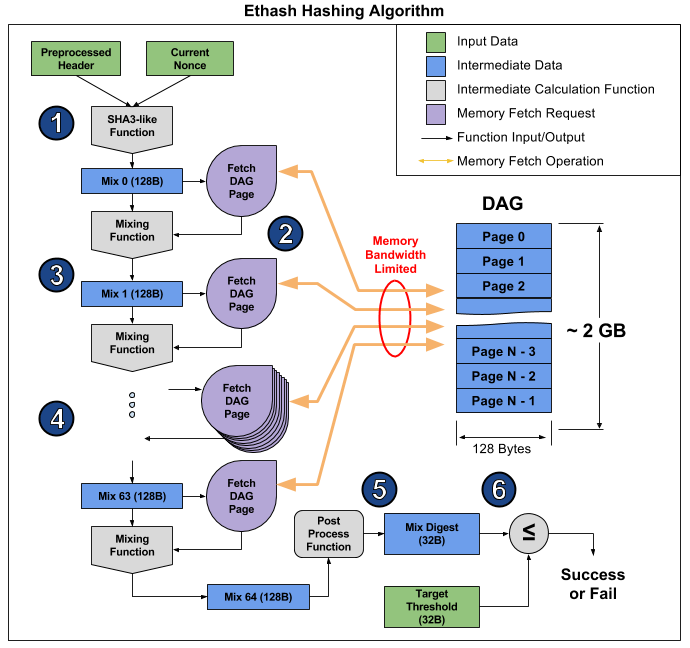
\includegraphics[width=300px,keepaspectratio]{ethash_algorithm.png}
\caption{\label{fig:ethash} Ethash}
\end{figure}


\section{Our Approach}
We propose a lazy-evaluation based approach to alleviate the network and memory requirements for mining ethereum in a distributed scenario on browsers. Specifically, as soon as each browser connects to the webserver, the server sends it the current header of the block being mined and the Cache. Once the browser receives the Cache, it allocates an array buffer to store the DAG slices that will be computed in the future. (Note that the length of the buffer is a variable parameter that we experiment with in our analysis). Once this happens, the browser can start iterating over nonces to compute hashes.  

Since, to begin with, the browser does not have any slices of the DAG, it must compute each slice on the fly using the Cache. However, for every such slice that the browser computes, it then stores it in the buffer (if it fits within the allocated bounds, otherwise it is simply discarded), for quicker access in the future. Hence, as time passes, the buffer starts filling up and so more and more slices are quickly accessed from the buffer rather than being computed from the ground-up, which makes hash computations faster with time. This has the effect that the longer the user remains on the web-page, the better the hashrate gets for that user. 

\subsection{Information theoretic bounds}
With this lazy-evaluation based approach, we can calculate exactly how many hashes we would have to compute in order to fill up a buffer of a given size. This is important because once the buffer in the browser fills up, the hashrate that the browser gives becomes steady. Hence, calculating the expected number of hashes it takes to fill the buffer allows us to determine how much time will the browser take to reach a steady state hash rate. This approach is a variation of the coupon collector problem \cite{couponCollector}, and has been described in the following theorem: 
\begin{theorem}[Expectation of Number of Hashes]
\label{expectedHashes}\\
If we define,
    \[Number\;of\;DAG\;slices\;=\;n\]
    \[Size\;of\;buffer\;as\;a\;fraction\;of\;the\;total\;DAG\;=\;f_1;\;f_1=[0,1] \]
    \[Expected\;number\;of\;hashes\;it\;takes\;to\;fill\;the\;buffer\;= E(H)\]
Then the expected number of hashes $E(H)$ it takes to fill up a buffer of fraction $f_1$ of a DAG with $n$ slices is given by:
\begin{gather}
E(H) = \frac{n\log{nf_1}}{64}
\end{gather}
\end{theorem}
\begin{proof}
Let us assume we have a buffer for our DAG that is $f_1$ as large as the entire DAG -- i.e., the buffer can only store dag slices with indices $i$ such that $i \in [0,nf_1]$. Hence, each time we calculate a DAG slice from the Cache, we may or may not buffer it depending on whether it falls within the index rage. Now, let us assume that  we have buffered $x$ slices so far, the probability of obtaining a new slice is given by:
\begin{gather}
  P_x = \frac{nf_1-x}{n}
\end{gather}
The event of obtaining a new slice after having already collected $x$ out of the $nf_1$ slices that can be buffered can be modeled as a geometric distribution. Hence, the expected number of trials $t_x$ it takes to get a new  slice after having seen $x$ out of the $nf_1$ slices is:
\begin{gather}
  E(t_x) = \frac{1}{P_x} = \frac{n}{nf_1-x}
\end{gather}
By linearity of expectation, the total number of trials it would take to see all $x$ slices is:
\begin{gather}
  E(t) = \sum_{x=0}^{nf_1-1}E(t_x) = \sum_{x=0}^{nf_1-1}P_x = \sum_{x=0}^{nf_1-1}\frac{n}{nf_1-x} = n\sum_{x=0}^{nf_1-1}\frac{1}{nf_1-x}
\end{gather}
Since the summation represents the harmonic series, the expected value can be approximated as follows:
\begin{gather}
  E(t) = n\log{nf_1}
\end{gather}
Equation ~\ref{eq:7} is in terms of the number of individual accesses of the DAG. In order to get the expected number of Hashes (as opposed to the expected number of individual DAG slice accesses), we need to divide by 64 since each hash involves 64 accesses of the DAG. Hence: 
\begin{gather}
  E(H) = \frac{E(t)}{64} = \frac{n\log{nf_1}}{64}
\end{gather}
\end{proof}
Now, let us do a simple calculation for one extreme case, where $f_1 = 1$ (i.e., we allocate a buffer as large as the entire DAG on the browser), in order to get an upper bound on the number of hashes it would take to fill this buffer up. The private test network for Ethereum we used had a total of 16777186 slices in the DAG, which means it would take:
\begin{gather}
  E(H) = \frac{16777186*\log{16777186}}{64} = 4.36*10^6\;hashes
\end{gather}
Hence, it takes around 4 million hashes to fill up a buffer as large as the entire DAG. If $f_1 < 1$, the number of hashes should be less than 4 million. So effectively, 4 million hashes is a very lose upper bound on the number of hashes needed to fill up a DAG buffer. However, since 4 million hashes can be a lot for a browser, we will now demonstrate how we can get away with  better

Now let us say that we do not want to wait for the entire buffer to fill up -- how many hashes would we have to compute until a reasonable fraction of the buffer is full? For this, we have the following corollary:
\begin{corollary}
\label{earlyTermination}
If we define,
  \[Fraction\;of\;DAG\;buffer\;to\;be\;filled = f_2;\;f_2 \in [0,1]\]
  Then,
    \begin{gather}
    E(H) = \frac{n}{64}\log{\frac{1}{1-f_2-\frac{1}{nf_1}}}
  \end{gather}
\end{corollary}
\begin{proof}
Then, for a buffer with space for $f_1$ slices, the number of slices we want to fill it with in order for a fraction $f_2$ of it to be full would be: 
\begin{gather}
  Number\;of\;slices\;to\;fill\;DAG\;buffer\;with = nf_2f_1
\end{gather}
This would modify equation \ref{eq:6} for the expected number of trials to fill up a fraction $f_2$ of the DAG buffer to be as follows:
\begin{gather}
    E(t) = \sum_{x=0}^{nf_2f_1}P_x = \sum_{x=0}^{nf_2f_1}\frac{n}{nf_1-x} = n\sum_{x=0}^{nf_2f_1}\frac{1}{nf_1-x}
\end{gather}
This is essentially an early termination of the summation in equation ~\ref{eq:6}, and can be expressed as follows:
\begin{gather}
    E(t) = n\sum_{x=0}^{nf_2f_1}\frac{1}{nf_1-x} = n(\sum_{x=0}^{nf_1-1}\frac{1}{nf_1-x} - \sum_{x=nf_2f_1+1}^{nf_1-1}\frac{1}{nf_1-x})\\
    E(t) = n(\log{nf_1} - \log{(nf_1-nf_2f_1-1)}) \\
    E(t) = n\log{\frac{1}{1-f_2-\frac{1}{nf_1}}}
\end{gather}
Again, we divide by 64 to obtain the expected number of hash computations:
\begin{gather}
    E(H) = \frac{n}{64}\log{\frac{1}{1-f_2-\frac{1}{nf_1}}}
\end{gather}
\end{proof}
Interestingly, since for realistic cases $n >> f_1$, $\frac{1}{nf_1} \to 0$, and so 
\begin{gather}
E(H) \approx \frac{n}{64}\log{\frac{1}{1-f_2}}
\end{gather}
Figure X shows a graph of how $E(H)$ varies as a function of the fraction of the buffer that we want to be full, $f$ if we set $n = 16777186$ (the total number of DAG slices on the experimental private test network). 

From figure X we see that even computing merely 800,000 hashes fills our DAG buffer by more than 95\%, as opposed to calculating 4 million to fill the buffer entirely. This suggests that the fuller the buffer is, the marginal cost of computing more hashes outweighs the rate at which the buffer is filled up. This also means that reaching a reasonably steady state is not as hard as it seems at face value. Given this result, we compute 800,000 hashes for our experiments.
% Beyond that, the marginal cost of computing more hashes outweighs the rate at which the DAG is filled up. Hence, as we will see in the next section, for our experiments, we compute 800,000 hashes.

\section{Architecture}
% \begin{figure}[H]
% \centering
% \includegraphics[width=250px,keepaspectratio]{miningpool.png}
% \caption{\label{fig:miningpool} Distributed Ethereum Mining}
% \end{figure}

Our architecture was centered around two client-side Ethereum miners written in \verb|JavaScript| and \verb|WebAssembly|. The central node that co-ordinates all workers (browsers) was an improvised version of \verb|geth| ~\cite{geth}, a real world Ethereum miner written in \verb|Go|. \verb|Geth| typically runs as a standalone miner that mines on the machine it is running. We modified it so that instead of mining all by itself, it simply sends over the necessary data needed to mine (the hash of the Block Header and the Cache) to any client that connects to it on port \verb|9000|. After recieving the necessary data, the browser allocates a buffer for the DAG in order to store future slices. Note that the buffer for the DAG is implemented an array of ints (with a DAG slice being 16 ints long), so as to make each lookup in the buffer $\theta(1)$. At this point, it can then begin to search for a solution. 

For our miner, we modeled our \verb|JavaScript| implementation based on the ~\verb|node.js| implementation of Ethash ~\cite{ethash}. To begin, the miner creates a random nonce and the computes the hash (using the Cache and the buffered DAG) as discussed in the previous section. It will continue to perform this action on new nonces until one of two scenarios occur; it finds a nonce such that the computed hash is below the given threshold or the process has timed out. In the former case, the browser submits the result back to the node and then asks the node for a new block header and the Cache. Otherwise if it has timed out without finding a result, the browser simply polls the node for the current block header and Cache . This process will continue until the user moves away from the website or closes their browser. 
We must point out that this time out is necessary since we want the browser to work with the most recent block header and Cache. The block header can become stale if that particular block has already been mined, and the Cache can become stale if the Ethereum network transitions into a new Epoch (happens once every 30,000 blocks). 
We must point out that both our current implementations in \verb|JavaScript| and \verb|WebAssembly| require no external dependencies, and therefore can be directly embedded into any website. For a diagramatic view our our design, see Figures~\ref{fig:hybridArchitecture}.

\begin{figure}[H]
\centering
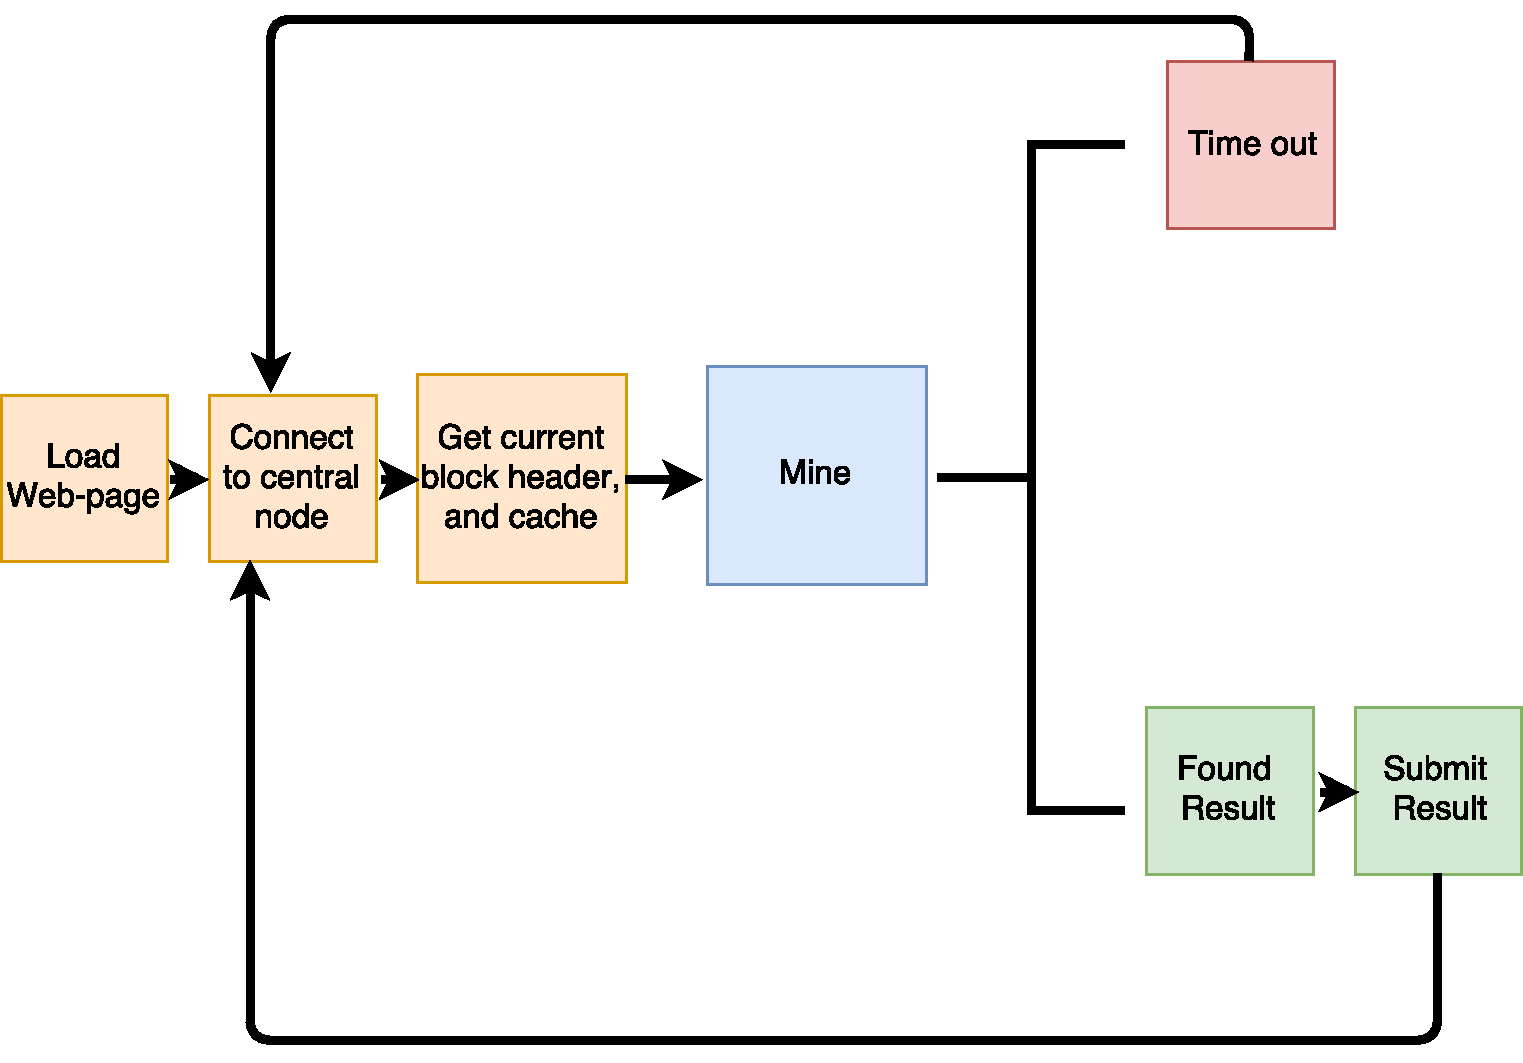
\includegraphics[width=250px,keepaspectratio]{Hybrid-Miner.pdf}
\caption{\label{fig:hybridArchitecture} Web Miner Architecture}
\end{figure}

\section{Results}
\subsection{Experimental set up}
Our experimental set up consisted of a machine with an Intel i7-7700HQ processor with 4 cores and 16GB ram. These results were obtained from a private Ethereum test network at Epoch 0. The DAG size was 16777186 slices (with each slice being a sequence of 16 ints). The cache size was X.

\subsection{Baseline results}
For our control results, we ran \verb|Geth|~\cite{geth}, a native miner written in \verb|Go| that stores the entire DAG in memory from the start (as opposed to using this lazy evaluation approach), and obtained an average hashrate of X H/s. We also ran our lazy-evaluation based miner written in C++ outside of the browser, and obtained the following results. 
Figure X below shows a heat-map of how the hash rate varies as a function of both the size of the buffer allocated to store the DAG (as a percentage of the size of the entire DAG) and the number of hashes computed in the browser. Figures X then shows a heat-map of how the DAG buffer hit-rate varies as a function of both the size of the buffer allocated to store the DAG and the number of hashes computed in the browser. 

% . Since the hashrate determines how fast a mining rig can verify a nonce, it was necessary to ensure that our results were not skewed due to the differences in computing power between computers. Using this machine, we recorded the hashrates for CPU performance and GPU performance on our private Ethereum testnet. 
% Additionally, we also recorded the hashrates for CPU mining in a Kali Linux VM. As we can see in the figure below, the GPU clearly outperforms the CPUs resulting in an average hashrate of 5.72MH/s. As for the CPUs, both miners performed about the same, both hovering around a respectable 210kH/s.
% \begin{figure}[H]
% \centering
% \includegraphics[width=250px,keepaspectratio]{GPU.png}
% \caption{\label{fig:gpu} GPU vs CPU Hashrates}
% \end{figure}

% \begin{figure}[H]
% \centering
% \includegraphics[width=250px,keepaspectratio]{CPU.png}
% \caption{\label{fig:cpu} VM CPU vs CPU Hashrates}
% \end{figure}

\subsection{Implementation Results}

% This happens because as described before, for the hybrid implementation where we store a small part of the DAG, we had to store the DAG in a \verb|javascript| object (Hash Map), with the ``keys'' being the index of the DAG and the value being the 512 bit slice that corresponds to that index. However, key-value look up times with \verb|JavaScript| objects are slow, according to the V8 design documentation for the language: ``Most JavaScript engines use a dictionary-like data structure as storage for object properties - each property access requires a dynamic lookup to resolve the property's location in memory. This approach makes accessing properties in JavaScript typically much slower than accessing instance variables in programming languages like Java and Smalltalk.'' ~\cite{AttrLookupLatency} This explains why storing larger and larger chunks of the DAG gives worse Hash rates, since it takes longer and longer to look up the required slices from the Hash Map. Indeed, this is why not storing the DAG at all, and just computing the slices from the Cache gives a high hash rate of \~ 1500 hashes/sec. The other extreme -- storing the entire DAG in memory is also slow because it takes up a lot of memory on the client's system. 

Note that this is the computational power of one machine and in reality, there would be hundreds or thousands of machines mining simultaneously, which will be analyzed in the next section. In comparison to Monero or Bitcoin browser miners who mine on an average of about 30-60H/s, our hashrate is significantly better than those.

\subsection{Difference Between Baseline and Implementation}
We see that the average hashrate outperforms.

One way to reach the steady state hashrate faster for a given sized buffer would be to start out with a partially filled out buffer instead of an empty one. The only way this could work is by sending over part of the DAG over the network to the client. However, as it turns out, this is not feasible since, for a DAG with 16777186 slices (1.074 GB) sending even 10\% of the DAG would be sending \~100MB of data. With the global average download speed for desktops and smartphones being around 5.34MBps and 2.77MBps respectively ~\cite{http://www.speedtest.net/global-index}, the load time would be on the order of 20 seconds to a minute -- which is too long a webpage load time for getting a mere 10\% boost in the buffer storage. 

\section{Future Work}

While we were able to create a browser based miner for Ethereum, there is still work to be done. As was shown, our current implementation is far slower than the traditional methods for mining. One way we can look to speed this process up is to tap into the client machine's GPU. There is a \verb|JavaScript| library called WebCL that binds to the OpenCL library which allows the \verb|JavaScript| to speak directly to the GPU for better parallel performance. Knowing that Ethereum was created for GPU mining and based on our results, it should provide a substantial improvement. 
% In addition, because of the memory hard requirements of the Ethereum protocol we should also see a better performance if we can somehow get the DAG to be directly accessible to the client instead of having to send slices over the network to all the clients. Therefore, we want to look into the use of \verb|remoteStorage| ~\cite{remote}, which allows the user to have complete control over the data. By moving the data closer to the computation we are hoping to cut the added time caused by the network.

Ethereum is also currently working on Casper, their Proof-of-Stake algorithm, which has already been deployed to private testnets for testing. Working with that and the fact that Casper is open-source, it would be possible to create a theoretical Proof-of-Stake distributed browser miner implementation in preparation for the fork. However, seeing as though Proof-of-Stake would virtually eliminate the necessity of massive amounts of processing power, users would most likely have to provide ``stakes" in order for such an implementation to be possible ~\cite{PoSproof}. Further research will be necessary to determine whether browser mining for Casper is viable or not, as the final form of Casper is still hazy and exactly how much ``stake'' is required to mine is uncertain.


\section{Conclusion}
We have successfully created a proof of concept distributed, web-based Ethereum miner that can be used towards monetizing electronic content. Our implementation is standalone, and hence can simply be embedded within a website without having the client install any external dependencies. Furthermore, we provide an API that can be used by any implementation of Ethereum (\verb|geth| or Ethereum's implementation in \verb|C++|). We believe this can be a be especially viable in a private testnet, within a company for example, and with further research has the potential to make a real impact.

% conference papers do not normally have an appendix


% % use section* for acknowledgement
\section*{Acknowledgment}
The authors would like to thank Dennis Your for his contributions to this work.

\begin{thebibliography}{1}
\bibitem{Adblock} Gundlach, Micheal. AdBlock browser extension. AdBlock. Software, 2009.

\bibitem{ethash}Matthew Wampler, et al. Ethash. Computer software. GitHub. Vers. 23.1. GitHub, 11 Jan. 2015. Web. 24 Feb. 2018. <https://github.com/ethereum/ethash>. 

\bibitem{BraveBrowser} Eich, Brendan and Brian Bondy. Brave Browser. Brave Software. Software, 2015.

\bibitem{decliningRevenue} Hern, Alex. “Adblock Plus: the Tiny Plugin Threatening the Internet's Business Model.” The Guardian, Guardian News and Media, 14 Oct. 2013, www.theguardian.com/technology/2013/oct/14/the-tiny-german-company-threatening-the-internets-business-model.

\bibitem{dagger-hashimoto} Buterin, Vitalik, et al. “Ethereum/Wiki.” GitHub, GitHub, 9 Feb. 2014, github.com/ethereum/wiki/blob/master/Dagger-Hashimoto.md. 

\bibitem{noSubscriptions} Rosenwald, Micheal. “Digital News Consumers Unlikely to Pay for Content and Increasingly Block Ads.” Columbia Journalism Review, Columbia Journalism Review, 15 June 2015, www.cjr.org/analysis/reuters\_digital\_news\_report.php.

\bibitem{payPerClick} Fessenden, Therese. “Nielsen Norman Group.” The Most Hated Online Advertising Techniques, Nielsen Norman Group, 4 June 2017, www.nngroup.com/articles/most-hated-advertising-techniques/.

\bibitem{celebEndorse} Awad, Amal. “A Study in Scarlett: The Ethics of Celebrity Endorsement.” – Opinion – ABC Religion \&Amp; Ethics (Australian Broadcasting Corporation), Amal Awad ABC Religion and Ethics, 30 Jan. 2014, www.abc.net.au/religion/articles/2014/01/31/3935443.htm.

% \bibitem{Boldrin} Boldrin, F., et al. “Distributed Computing Through Web Browser.” Distributed Computing Through Web Browser - IEEE Conference Publication, University of Ferrara, ieeexplore.ieee.org/document/4350073/.

\bibitem{scheduling}
Ramamritham, Krithi, and John A. Stankovic. "Dynamic task scheduling in hard real-time distributed systems." IEEE software 1.3 (1984): 65.

\bibitem{parallel}
Shirazi, Behrooz A., Krishna M. Kavi, and Ali R. Hurson. Scheduling and load balancing in parallel and distributed systems. IEEE Computer Society Press, 1995.

\bibitem{orca}
Bal, Henri E., M. Frans Kaashoek, and Andrew S. Tanenbaum. "Orca: A language for parallel programming of distributed systems." IEEE transactions on software engineering 18.3 (1992): 190-205.

\bibitem{WebFlow}
Bhatia, Dimple; Burzevski, Vanco; Camuseva, Maja; and Fox, Geoffrey C., "WebFlow - A Visual Programming Paradigm for Web/Java Based Coarse Grain Distributed Computing" (1997).
Northeast Parallel Architecture Center.

\bibitem{Cushing} Cushing, Reginald, et al. “Distributed Computing on an Ensemble of Browsers.” IEEE Internet Computing, IEEE, 1 Sept. 2013, www.computer.org/csdl/mags/ic/2013/05/mic2013050054.html.

\bibitem{randmemohash} Lerner, Sergio Demian. "STRICT MEMORY HARD HASHING FUNCTIONS (PRELIMINARY V0. 3, 01-19-14)."

\bibitem{coinhive}
The Coinhive Team. Coinhive browser extension. Coinhive. Software, 2017.

\bibitem{pow}
Laurie, Ben, and Richard Clayton. "Proof-of-work proves not to work; version 0.2." Workshop on Economics and Information, Security. 2004.

\bibitem{casper}
Hertig, Alyssa. “Ethereum's Big Switch: The New Roadmap to Proof-of-Stake.” CoinDesk, CoinDesk, 16 May 2017, www.coindesk.com/ethereums-big-switch-the-new-roadmap-to-proof-of-stake/. 

\bibitem{pos}
Dmitry Buterin, et al. “Proof of Work vs Proof of Stake: Basic Mining Guide.” Blockgeeks, Blockgeeks, 24 July 2017, blockgeeks.com/guides/proof-of-work-vs-proof-of-stake/. 

\bibitem{arc}
The ArcticCoin Team. ArcticCoin crypto-currency. ArcticCoin. Software, 2015.

\bibitem{Monero} “Monero - Secure, Private, Untraceable.” Getmonero.org, The Monero Project, getmonero.org/.

\bibitem{Duda} Duda, Jerzy, and Wojciech Dłubacz. “Distributed Evolutionary Computing System Based on Web Browsers with Javascript.” ACM Digital Library, Springer-Verlag, dl.acm.org/citation.cfm?id=2451764.2451780.

\bibitem{traffic} The SimilarWeb Team. SimilarWeb LTD 2017. (https://www.similarweb.com/)

\bibitem{coinwarz}Coinwarz Ethereum Mining Calculator and Profit Calculator. Coinwarz 2017. (https://www.coinwarz.com/calculators/ethereum-mining-calculator)

\bibitem{PoSproof}Dale, Oliver. "Beginner's Guide to Ethereum Casper Hardfork: What You Need to Know". Blocknomi, 7 November 2017. (https://blockonomi.com/ethereum-casper/)

\bibitem{Ethmining}
Wood, Gavin. "Ethereum: A secure decentralised generalised transaction ledger." Ethereum Project Yellow Paper 151 (2014): 1-32.

\bibitem{geth}Péter Szilágyi, et al. Geth. Computer software. GitHub. Vers. 1.8.1. GitHub, 22 Dec. 2013. Web. 24 Feb. 2018. <https://github.com/ethereum/go-ethereum>. 

\bibitem{etherscan}Etherscan The Ethereum Block Explorer. Etherscan 2017. (https://etherscan.io/charts)

\bibitem{remote} remoteStorage: An open protocol for per-user storage on the Web. (https://remotestorage.io/)
\end{thebibliography}

\addtolength{\textheight}{-7cm}
\balance


% that's all folks
\end{document}